%---------------------------------------------------
%---------------------------------------------------
%-----   COPY FROM HERE TO DEFINITIVE FILE    ------
%---------------------------------------------------
%---------------------------------------------------

\clearpage{\pagestyle{empty}\cleardoublepage}

\chapter{Physics beyond the Standard Model}\label{chap:bsm}
Up to now, the Standard Model (SM) is the most beautyful and precise theory explaining the world of particle physics but it is far from being complete: indeed the SM without the Higgs boson predicts massless fermions and gauge bosons and that's the reason why so much spotlight is put on LHC's hunt for the Higgs boson. Moreover, the SM has some theoretical problems that can be solved only by an extension in the theory, going into new physics like Supersymmetry (SUSY). However the excellent consistency between data and model makes the SM, at least, an extremely accurate theory for energy scale up to a few hundred of GeV, even though it is likely to become only an approximation of a more complete theoretical framework.


\section{Standard Model: building and confirmations}
During the first half of the 20th century, many experimental discoveries were challenging particle physicists to find a coherent model to explain the existence of new particles and forces. A ``heavy electron'', the muon, was observed in 1936 by Carl Anderson in cosmic radiation. The neutrino, postulated by Wolfgang Pauli to explain the shape of the electron spectrum in beta decay, was experimentally detected in 1956 by Clyde L. Cowan and Frederick Reines, and few years later a second neutrino type was discovered by Leon M. Lederman, Melvin Schwartz and Jack Steinberger. By 1963 a huge number of new mesons and baryons were populating what was called the ``particle zoo'' until Murray Gell-Mann and George Zweig independently found a classification for all these new particles supposing that hadrons were made by smaller components (Figure \ref{eightfold}). It was the beginning of the quark model, a theory that had to wait for multiple experimental evidence before being accepted. Even when in 1968 deep inelastic experiments at the Stanford Linear Accelerator Center (SLAC) found out evidence for a substructure in protons, physicists were reluctant to accept this point-like objects to be quarks. Richard Feynman called them \textit{partons}, the term now used to identify quarks and antiquarks as well as gluons.

\begin{figure}[htb]\begin{center}
\includegraphics[width=.7\textwidth]{./capBSM/eightfold}\caption{Gell-Mann's \textit{Eightfold Way} for mesons (a) and baryons (b), classified through their electric charge and strangeness (from \cite{Nature74}). The Eightfold Way model (proposed also independently by Yuval Ne'eman) organizes spin-zero mesons and spin-half baryons into octets and spin-3/2 baryons into a decuplet with a strangeness-(-3) particle $\Omega^{-}$ predicted in 1962 and discovered in 1964 at Brookhaven. Born as a classification in terms of electric charge $q$ and strangeness $s$, it is now understood that it is a consequence of flavour symmetry.}
\label{eightfold}\end{center}\end{figure}

However, there was a bigger problem tormenting theoretical physicists. Quantum field theory was in fact apparently unsuitable for the description of the dynamics of particles interactions, since divergences appeared in the high energy domain. In 1954 Chen N. Yang and Robert Mills proposed a new gauge theory based on the principle of local gauge invariance i.e. the property of space-time regions of not being affected by a symmetry transformation performed locally in a different region. With the addition of a scalar field by Peter Higgs, Fran\c{c}ois Englert and Robert Brout and the implied modification of the vacuum structure (see Section \ref{sect:higgs} for more details), the Yang-Mills field became a very accurate description of the weak force interactions. Such model was consistently proposed in the 1960s by Abdus Salam, Sheldon Glashow and Steven Weinberg, but it suffered of a problem: as it was a perturbative theory, equations had to be expanded in a power series to be calculated but only the leading order term did not show ultraviolet divergences.

By the first years of the 1970s Martinus Veltman and Gerard't Hooft demonstrated renormalization for the theory, with the result that divergences could be cancelled and physical observables obtained with precisions higher than the leading order. 
%The concept of \textit{renormalization group} was needed to study the behaviour of the theory over short distances and the $\beta$-function, a function introduced by Curtis Callan and Kurt Symanzik and present in every theory, was the key of the understanding of such behaviour. In fact, a positive $\beta$ leads to an increasing coupling strenght at short distances, while a negative $\beta$ means that forces are weakened when reducing distance. It was a kind of suprise to discover that for Yang-Mills theories $\beta$ is generally negative, since it was believed that gauge theories had always a positive $\beta$-function. This was the discovery of \textit{asymptotic freedom}, a property that made Yang-Mills theory suitable also to describe strong interactions and that matched properly with the experimental effect named \textit{Bjorken scaling}\footnote{At SLAC it was observed during deep inelastic scattering experiments that strong interactions show a decrease of strenght at short distances (i.e. high momentum transfer) together with a scaling behaviour. A property is said to ``scale'' when it depends only by dimensionless kinematic quantities, such as a scattering angle or the ratio of the energy to a momentum transfer.}. 
The concept of \textit{renormalization group} was introduced and Yang-Mills theories were found to have a $\beta$-function (a function typical of gauge theories) generally negative. This was the discovery of \textit{asymptotic freedom}, a property that made Yang-Mills theory suitable also to describe strong interactions and that matched properly with the experimental effect named \textit{Bjorken scaling}\footnote{At SLAC it was observed during deep inelastic scattering experiments that strong interactions show a decrease of strenght at short distances (i.e. high momentum transfer) together with a scaling behaviour. A property is said to ``scale'' when it depends only by dimensionless kinematic quantities, such as a scattering angle or the ratio of the energy to a momentum transfer.}. 

At the same time, the three-quark model by Gell-Mann and Zweig was about to be expanded. In 1963 Nicola Cabibbo proposed the mixing of up, down and strange quark in order to explain the non-conservation of quark flavour in weak interactions as $\Lambda \rightarrow p^{+}\pi^{-}$ with $\Delta S$=1 and the empirical law $\Delta S = \Delta Q$ for strangeness changing processes. In 1970 Glashow, John Iliopoulos and Luciano Maiani (GIM) predicted a fourth quark, the charm, to account for the non observation of Strangeness Changing Neutral Current (SCNC) processes. Thus, the Cabibbo-GIM matrix $2\times 2$ parameterized by the Cabibbo angle $\theta_{C}$ described the quark mixing between these two families:
\begin{equation}\label{CabibboGIM}
V_{c} = {\setlength\arraycolsep{6pt}
\left( \begin{array}{cc}
\cos\theta_{C} & \sin\theta_{C}\\
-\sin\theta_{C}& \cos\theta_{C}
\end{array}
\right)} \quad .
\end{equation}
Furthermore, after the observation of CP violation events, Makoto Kobayashi and Toshihide Maskawa supposed the existence of two more quarks, the bottom and the top, thus increasing the number of quark flavours to six. This allowed the introduction in the new $3\times 3$ mixing matrix (the Cabibbo Kobayashi Maskawa CKM matrix) of, besides three angles, a complex phase that is responsible of CP violation. All this conjectures found an important confirmation in November 1974, known as the November Revolution maybe beacuse it was the beginning of a real trust in quark theory. Almost simultaneously at SLAC and at Brookhaven the charm quark was discovered in the bound state $c\bar c$, called $J$ meson by the Brookhaven team and $\psi$ by the SLAC one, so that in the end it was named $J/\psi$. Bottom quark was observed in 1977 at Fermilab, enhancing the belief in the top quark existence and in the six flavours theory.

The discovery of the tau lepton in 1978 and of the $W$ and $Z$ bosons in 1983 finally set the scene for the SM. Table \ref{tab:SM} shows the three generations of fermions, each of them having an antiparticle, and the three forces (three Yang-Mills fields) with their carriers composing the SM. A great achievement of the SM was the unification of electromagnetic and weak theories in the Electroweak Theory by Salam, Glashow and Weinberg. In fact, since at a scale of about 100 GeV the coupling constants converge, it is possible to describe them within the same mathematical model. Quantum ChromoDynamics (QCD) instead describes the strong interaction in terms of the color threefold charge and up to now is not known if also the strong coupling constant can become equal to the others at some high energy scale. However, a unified theory is strongly desired, as will be explained in Section \ref{sect:whyBSM}.
\begin{table}[htb]\centering\begin{tabular}{ccc|cc}
&\multicolumn{2}{c}{Leptons}&\multicolumn{2}{c}{Quarks} \\ 
& $q=-1$ & $q=0$ &$q=2/3$ &$q=-1/3$ \\ \hline
I & $e^{-}$ & $\nu_{e}$ & $u$ & $d$ \\
II & $\mu^{-}$ & $\nu_{\mu}$ & $c$ & $s$ \\
III & $\tau^{-}$ & $\nu_{\tau}$ & $t$ & $b$ \\\hline\hline
Force & Elm &\multicolumn{2}{c}{Weak}& Strong\\
Carrier & $\gamma$ & \multicolumn{2}{c}{$W^{\pm}$ \quad $Z$} & $g$\\\hline \hline
\end{tabular}\caption{Elementary particles and forces of the SM.}\label{tab:SM} \end{table}

Even if SM was born to be merely a stepping stone, it consolidated through years, standing all experimental tests sometimes with a precision greater than 0.1\%. Experiments carried out at LEP, thanks to the clean signals given by $e^{+}e^{-}$ collision events, allowed to obtain very high precision measurements of SM parameters. In particular experiments ALEPH, DELPHI, L3 and OPAL performed the measurements of the $Z$ boson mass with a precision of 0.0023\% that made it one of the most precisely known quantities within the SM\footnote{Note that the masses of the $W$ and $Z$ bosons are not predicted by the theory, but their ratio is (see Section \ref{sect:higgs}).}. Furthermore, measurements of its total decay width and of its partial decay widths for all processes with a visible final state (i.e. different from $\nu\bar\nu$) allowed to set the number of light neutrino flavours to three, confirming the three-generation SM and excluding the possibility for a fourth family of leptons with masses lower than half of $m_Z$.

The last discovery inside the SM has been the observation of the top quark in 1995 at the Fermilab's experiments CDF and D0. The mass of the top quark resulted consistent with the predicted constraints, thus confirming the SM as an accurate framework. There is a missing piece, though, that could invalidate all the previous beautiful confirmations, since the Higgs mechanism (Section \ref{sect:higgs}) is a cornerstone for the SM: a moderately light Higgs boson is in fact needed for the self-consistency of the overall fit of data. At present a preferred value of 80 GeV for the Higgs mass is predicted from precision measurements, although the lower limit from direct searches is 114 GeV with an upper limit of 144 GeV at 95\% C.L. \cite{Renton} (Figure \ref{higgsMass}). However, there are almost no doubts about the overall consistency of the SM. Figure \ref{higgsMass} shows a comparison between high precision measurements and values obtained from the fit \cite{Renton}.

\begin{figure}[htb]\begin{center}
\includegraphics[width=.43\textwidth]{./capBSM/higgsMass}\hspace{.7cm}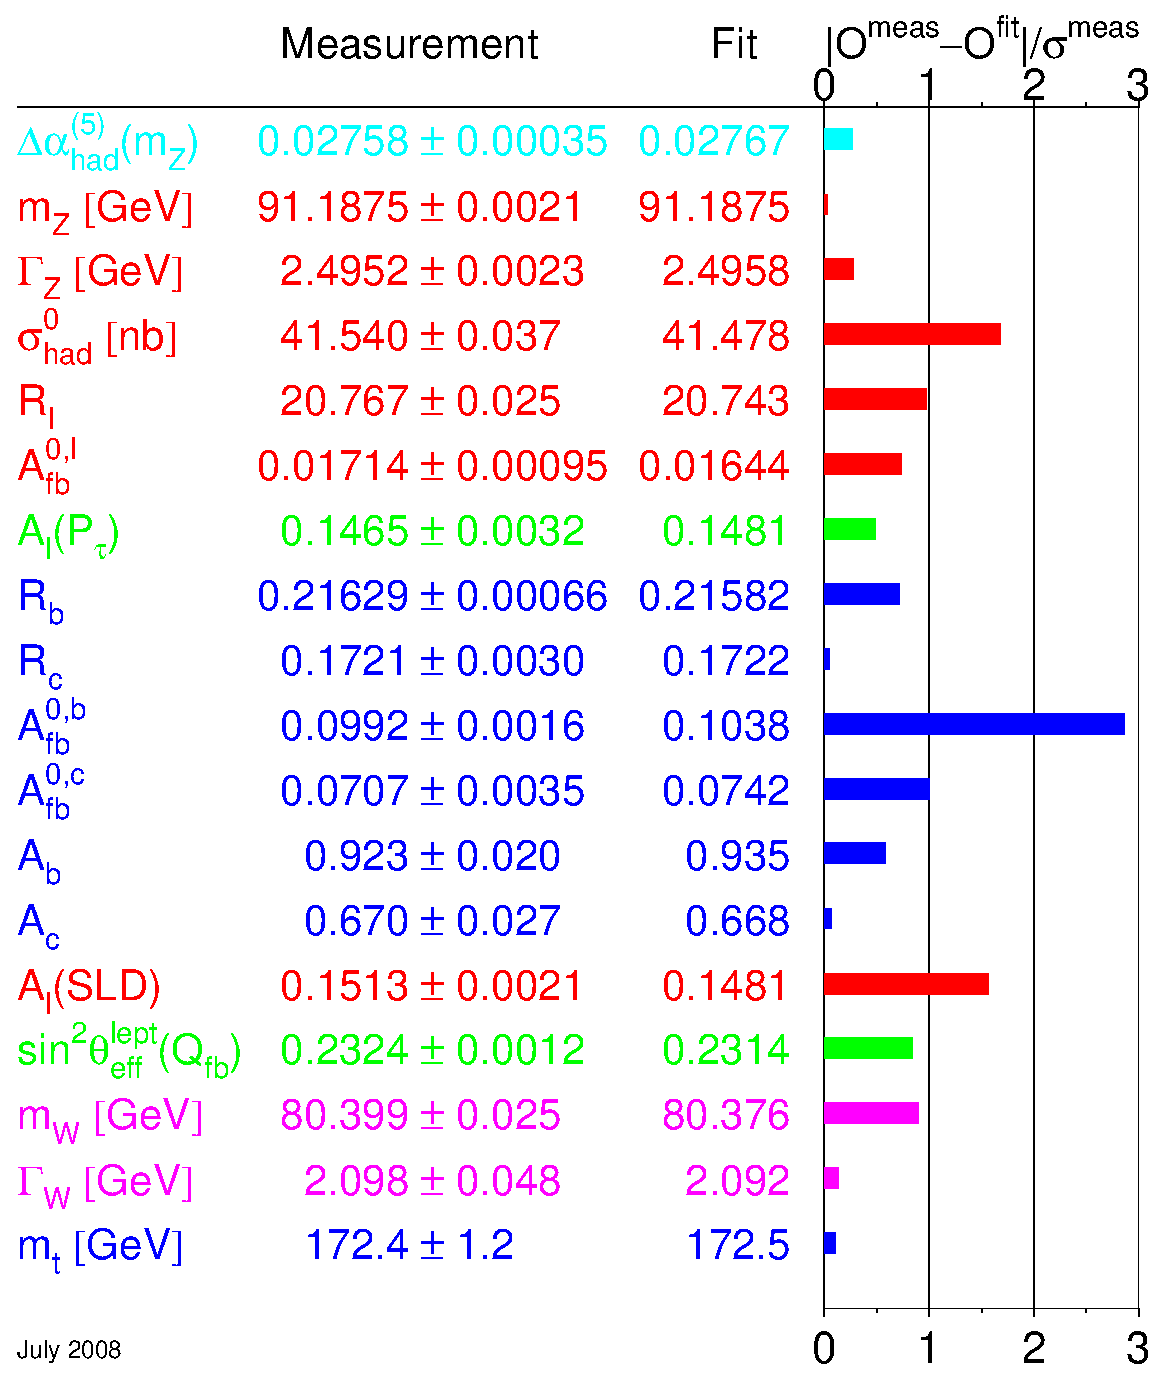
\includegraphics[width=.37\textwidth]{./capBSM/fitSM}\caption{Variation of the fit $\chi^2$ as a function of the Higgs mass with LEP2 excluded area (left) and a test of consistency of SM fit (right) \cite{Renton}.}
\label{higgsMass}\end{center}\end{figure}

\subsection{Standard Model Lagrangian and the Higgs Sector}\label{sect:higgs}
The Standard Model is a gauge theory invariant under the symmetry transformation $SU(2)_{L} \otimes U(1)_{Y}$. Using $\psi_{L}$ and $\psi_{R}$ to denote the left-handed and right-handed fermion fields respectively, the bare electroweak Lagrangian of the SM (considering for simplicity only leptons) is made of two terms\begin{equation}\label{eq:bareLagSM}
\mathcal{L}_{0} = \mathcal{L}_{lept}+ \mathcal{L}_{gauge}
\end{equation}that are \begin{align}
&\left \{ \begin{array}{ll}
\mathcal{L}_{lept} = \bar\psi_{L}i\slashed{D}_{L}\psi_{L} + \bar\psi_{R}i\slashed{D}_{R}\psi_{R}\\
D_{L}^{\mu} = \partial^{\mu} + ig\dfrac{\bar{\sigma}\cdot\bar{W}^{\mu}}{2} + i\dfrac{g'}{2}Y_{L}B^{\mu}\\
D_{R}^{\mu} = \partial^{\mu} + i\dfrac{g'}{2}Y_{R}B^{\mu}
\end{array} \right. ,\label{eq:lagLep} \\
&\left \{ \begin{array}{ll}
\mathcal{L}_{gauge}  = -\frac{1}{4}W_{\mu\nu}^{l}W^{\mu\nu\, l}  -\frac{1}{4}B_{\mu\nu}B^{\mu\nu}\\
B_{\mu\nu} = \partial_{\mu}B_{\nu} - \partial_{\nu}B_{\mu}\\
W_{\mu\nu}^{l} = \partial_{\mu}W_{\nu}^{l} - \partial_{\nu}W_{\mu}^{l} - g\varepsilon^{jkl}W_{\mu}^{j}W_{\nu}^{k}
\end{array} \right. .\label{eq:lagGauge}
\end{align}
Equation \ref{eq:lagLep} is the ``free matter'' Lagrangian after symmetries $SU(2)_{L}$ of isospin (with coupling constant $g$) and $U(1)_{Y}$ of hypercharge (with coupling constant $g'/2$) have been gauged through the definition of covariant derivatives, while equation \ref{eq:lagGauge} is the Lagrangian for the vector bosons dynamics. The chirality of the electroweak interactions does not find a theoretical motivation, but $SU(2)_{L} \otimes U(1)_{Y}$ transformations do make distinction between left and right helicity of the spinors:\begin{align}
&\left \{ \begin{array}{ll}
\psi_{L} = \frac{1}{2}(1 - \gamma_{5})\phi &\rightarrow \; \psi_{L}' = e^{iY\beta(x) + i\bar{\sigma}\bar{\alpha}(x)}\psi_{L} \\
\psi_{R} = \frac{1}{2}(1 + \gamma_{5})\phi &\rightarrow \; \psi_{R}' = e^{iY\beta(x)}\psi_{R}
\end{array} \right. .
\label{eq:chiral}
\end{align}

The Lagrangian \ref{eq:bareLagSM} is invariant under group $SU(2)_{L} \otimes U(1)_{Y}$ transformation, but has the problem of leaving fermions massless. Thus a scalar Lagrangian with a quartic auto-interaction is introduced:
\begin{equation}\label{eq:lagScalar}
\left \{ \begin{array}{ll}
\mathcal{L}_{\phi} =  (D_{\phi}^{\mu} \phi)^{\dag}(D_{\phi\,\mu} \phi) - V(\phi^{\dag}\phi)\\
V = \mu^{2}\phi^{\dag}\phi + \lambda(\phi^{\dag}\phi)^{2}\\
D_{\phi}^{\mu} = \partial^{\mu} + ig\dfrac{\bar{\sigma}\cdot\bar{W}^{\mu}}{2} + i\dfrac{g'}{2}Y_{\phi}B^{\mu}
\end{array}\right. ,
\end{equation}where $\phi$ is an Higgs doublet, accounting for four degrees of freedom:\begin{equation}\label{eq:higgsDoub}
\phi = \begin{pmatrix} \varphi^{+}\\\varphi^{0}
\end{pmatrix},\quad \varphi^{+}=\frac{1}{\sqrt{2}}(\varphi_{1}+i\varphi_{2}),\quad \varphi^{0}=\frac{1}{\sqrt{2}}(\varphi_{3}+i\varphi_{4}).
\end{equation}
Three terms, $\varphi^{+}$, $\varphi^{-}$ and $(\varphi^{0}-\bar\varphi^{0})/\sqrt{2}$, give mass to the three massive vector bosons $W^{\pm}$ and $Z$, leaving a massive Higgs scalar boson $(\varphi^{0}+\bar\varphi^{0})/\sqrt{2}$. Since now the fundamental vacuum state is no more invariant under $SU(2)_{L} \otimes U(1)_{Y}$, these two symmetries are now broken\footnote{Instead, the symmetry $U(1)_{elm} \subset SU(2)_{L} \otimes U(1)_{Y}$ is not broken. This means that vacuum is electrically uncharged while it has isospin and hypercharge charges.}: this is the Spontaneous Symmetry Breaking (SSB) mechanism. The vacuum state is chosen as\begin{equation}\label{eq:vacuum}
\phi_{0} = \begin{pmatrix} 0 \\ v/\sqrt{2}
\end{pmatrix}
\end{equation}where $v = \sqrt{-\mu^{2}/\lambda}$ is the vacuum expectation value. Finally, the only thing left to do is to introduce the scalar-fermion interaction. This is done with
\begin{equation}\label{eq:lagYukawa}
\mathcal{L}_{Yukawa} = -G_{lept}\big[\bar\psi_{R}(\phi^{\dag}\psi_{L}) + (\bar\psi_{L}\phi)\psi_{R}\big] .
\end{equation}Thus the complete electroweak Lagrangian of the SM, that can be generalized also to quarks (see Table \ref{tab:isospin}), is\begin{equation}\label{eq:lagSM}
\mathcal{L}= \mathcal{L}_{lept} +\mathcal{L}_{gauge} +\mathcal{L}_{\phi} +\mathcal{L}_{Yukawa}.
\end{equation}

\begin{table}[htb]\centering\begin{tabular}{cccc}
\multicolumn{4}{c}{Weak isospin left-handed doublets \bfseries $\psi_{L}$} \\ \hline \\ 
$\begin{pmatrix} \nu_{e_{L}} \\ e_{L} \end{pmatrix}$ & $\begin{pmatrix} \nu_{\mu_{L}} \\ \mu_{L} \end{pmatrix}$ &$\begin{pmatrix} \nu_{\tau_{L}} \\ \tau_{L} \end{pmatrix}$ & \bfseries Leptons \\ \\ 
$\begin{pmatrix} u_{L} \\ d'_{L} \end{pmatrix}$ & $\begin{pmatrix} c_{L} \\ s'_{L} \end{pmatrix}$ &$\begin{pmatrix} t_{L} \\ b'_{L} \end{pmatrix}$ & \bfseries Quarks \\
 \\ \hline \hline\\ 
\multicolumn{4}{c}{Weak isospin right-handed singlets \bfseries $\psi_{R}$} \\ \hline \\ 
$ e_{R} $ & $ \mu_{R}$ &$\tau_{R}$ & \bfseries Leptons \\ \\ 
$u_{R}$ , $d'_{R} $ & $c_{R}$ , $s'_{R} $ &$ t_{R}$ , $b'_{R}$ & \bfseries Quarks \\
 \\ \hline \hline
\end{tabular}\caption{Weak isospin multiplets. $q'$ refers to the flavour eigenstate that correspond to the mass eigenstate transformed with the CKM matrix.}\label{tab:isospin} \end{table}

An important consequence of the introduction of the scalar Higgs field is the mixing of the vector bosons $B^{\mu}$ and $W_{3}^{\mu}$ to give the photon $A^{\mu}$ and the $Z^{\mu}$ boson:\begin{equation}\label{eq:AZ}
\left \{ \begin{array}{ll}
A^{\mu} = \cos\theta_{W}B^{\mu} + \sin\theta_{W}W_{3}^{\mu}\\
Z^{\mu} = -\sin\theta_{W}B^{\mu} + \cos\theta_{W}W_{3}^{\mu}\end{array}\right. ,
\end{equation}where the Weinberg angle $\theta_{W}$ is defined through\begin{equation}\label{eq:weinb}
\left \{ \begin{array}{ll}
\dfrac{g}{\sqrt{(g')^{2}+g^{2}}} = \cos\theta_{W} \\
\dfrac{g'}{\sqrt{(g')^{2}+g^{2}}} = \sin\theta_{W} \end{array}\right. .
\end{equation} Masses acquired through the Higgs mechanism are listed in Table \ref{tab:mass}.
\begin{table}[htb]\centering\begin{tabular}{cccc}
\multicolumn{4}{c}{Force Carriers} \\ \midrule
$\gamma $ &$W^{\pm}$ &$Z$ &$g$ \\
$0$ & $\sqrt{\dfrac{g^{2}v^{2}}{4}} $& $\sqrt{\dfrac{(g^{2}+g'^{2})v^{2}}{4}} $&  $0$ \\
$0$ & $80.4$ & $91.2$ & $0$ \\\hline \hline\\
\end{tabular}

\begin{tabular}{cccccccccc}
\multicolumn{10}{c}{Leptons and Quarks} \\ \midrule
$e$ & $\mu$ &$\tau$ &$\nu$ & $u$ & $d$ & $c$ & $s$ &$ t$ & $b$ \\
\multicolumn{10}{c}{$\dfrac{v}{\sqrt{2}}g_{f}$} \\
$0.511\cdot10^{-3} $ & 0.105 & 1.777 & $\sim0$ & 0.0024 & 0.0048 & 1.27 & 0.104 & 171.2 & 4.2 \\\hline \hline
\end{tabular}\caption{Particle Masses in GeV.}\label{tab:mass} \end{table}

Adding the QCD (see e.g. \cite{Ecker} for more about QCD), the SM is finally described by the symmetry group $SU(2)_{L}\otimes U(1)_{Y}\otimes SU(3)_{C}$ with  $SU(2)_{L}$ containing the left-handed weak isospin doublets, $U(1)_{Y}$ containing the right-handed isospin singlets and $SU(3)_{C}$, the unbroken colour symmetry, containing the color triplets.

\section{The need to go Beyond the Standard Model}\label{sect:whyBSM}
The principal objection to the idea that the SM could be a final theory is the high number of parameters of the theory. In fact, 19 parameters are needed to fit data from experimental observations. 
Three of them  are the couplings of the gauge groups $g_3, g, g'$ also written as: \begin{equation}\label{eq:couplings}
\alpha_{s}=\dfrac{g_{3}^{2}}{4\pi} ,\quad \alpha_{elm} = \dfrac{e^{2}}{4\pi} =  \dfrac{g^{2}\sin^{2}\theta_{W}}{4\pi}, \quad \sin^{2}\theta_{W} = \dfrac{(g')^{2}}{g^{2}+(g')^{2}},
\end{equation}
13 parameters are associated with the nine charged fermion masses and the four parameters of the CKM matrix (three quark-mixing angles and one phase), two are needed to describe the SSB mechanism, i.e. the Higgs vacuum expectation value $v$ and the quartic coupling constant $\lambda$, and  finally one is the QCD $\theta$ parameter. Moreover, if neutrinos are massive (as it is almost certain from neutrino oscillation observations, see e.g. \cite{Langacker:817840}) there will be even more arbitrary parameters describing their masses and their mixing. Another disturbing feature of the model is the lack of theoretical explanation for the generations of quarks and leptons to be exactly three, and also the reason why particle masses are so different in order of magnitude is unknown.

Cosmology and cosmological observations also challenge the Standard Model. The reason for baryon-antibaryon asymmetry is still not understood although we know that it is connected to  CP violation. Besides, astronomical observations tell us that the energy density of the Universe is made only for a 4-5\% of ordinary baryonic matter, the other components being dark matter (20-25\%) and dark energy (70-76\%). Dark matter is non-baryonic matter that interacts only weakly and gravitationally. It is now believed that dark matter is composed  of Weakly Interacting Massive Particles (WIMPs) whose masses range from a few GeV to a few TeV and  are not predicted within SM. Dark energy instead is still more mysterious and maybe new physics will give some hints for its interpretation.

Another topic making the SM likely to need improvements is the desire to go further in the unification of theories. Gravity is not implemented in the SM being negligible at the electroweak scale of few hundreds of GeV, but it should become relevant going up to the Planck scale $\Lambda \sim 10^{19}$ GeV. Also, electroweak and strong forces forming the SM gauge group $SU(2)_{L}\otimes U(1)_{Y}\otimes SU(3)_{C}$ are expected to unify at high energy since their coupling constants are running constants dependent on the energy scale (Figure \ref{running}, $\alpha^{-1}_{i} = g^{2}_{i}/(4\pi)$). 
\begin{figure}[htb]\begin{center}
\includegraphics[width=.6\textwidth]{./capBSM/mssmsm}\caption{Running coupling constants in the SM and in the MSSM (see Section \ref{sect:susy}) as functions of the renormalization scale (from \cite{pdg2008}).}
\label{running}\end{center}\end{figure}
If, based on these considerations,  one assumes that the Standard Model is valid only up to  an energy scale $\Lambda$, the scalar Higgs boson mass\footnote{This argument does not apply to fermion masses which are protected by chiral symmetry, and that's the reason why fermion masses are said to be ``natural''.} should encounter radiative corrections from vacuum polarization diagrams (Figure \ref{topLoop}) of the order of $\Lambda$ giving to the mass the value \cite{dawson-1997} \begin{equation}\label{eq:higgsMass}
M_{H}^{2} \sim M_{H_{0}}^{2} + \dfrac{\lambda}{4\pi^{2}} \Lambda^{2} + \delta M_{H}^{2}. \end{equation}
If the mass counterterm $\delta M_{H}^{2}$ does not cancel the quadratically divergent contribution and if the cutoff scale is chosen as the Planck scale, then
\begin{equation}
M_{H}^{2} \sim 10^{32},\end{equation} i.e. $10^{28}$ times bigger than the experimentally expected value coherent with the SM and with the unitarity constraint. This argument is called the \textit{hierarchy problem}, and could be fixed within the SM by choosing a fine-tuned mass counterterm, a solution considered not really elegant also because fine tuning will be required for every order in the perturbative expansion.
\begin{figure}[htb]\begin{center}
\includegraphics[width=.2\textwidth]{./capBSM/topLoop}\caption{The typical vacuum polarization diagram for the Higgs is a top quark loop.}
\label{topLoop}\end{center}\end{figure}
%This argument looks the same of what made physicists pass from Fermi theory to SM. In fact at that time the Fermi point like interactions were a good description of weak scattering processes of fermions $f+f\rightarrow f+f$, but the unitarity  predicted that at an energy $E_{crit} \sim 600$ GeV the theory would become inconsistent. Then it was found that new physics (the vector bosons of the SM) was needed already from an energy scale about 100 GeV, maybe due to the small coupling constant of weak interaction. Now, the scattering process $W+W\rightarrow W+W$ has a scattering amplitude growing linearly to the self-coupling constant of the Higgs field $\lambda$. The formula for the critical energy is now related to the Higgs mass as \cite{Ho-Kim} $$\dfrac{E_{crit}}{v} = \exp\bigg(\dfrac{4\pi^{2}v^{2}}{3M_{H}^{2}}\bigg),$$ which for an higgs Higgs mass less than 150 GeV gives $E_{crit} \sim 10^{18}$, thus making the Higgs model valid up to that scale. However for an heavier Higgs with a mass about 700 GeV, such critical energy goes down to $10^{3}$ GeV.  It is to remark that in the electroweak interactions the Higgs contribution to radiative corrections is very low since is denoted by a logarithm function, thus giving low variations and not affecting the precision electroweak data. The meaning of this is, whatever the critical energy value will be, the SM is an effective theory embedded in a more fundamental theory with $E_{crit}$ acting as a cutoff.

\section{Supersymmetry and the Minimal SUSY extension of SM}\label{sect:susy}
In order to solve the hierarchy problem, a possible solution is to postulate the invariance of the theory under a symmetry operation which trasforms fermionic fields into bosonic fields (and viceversa), called \textit{supersymmetry}. In this theory to each fermionic or bosonic
degree of freedom of the SM is associated a ``superpartner''. These superpartners have all of the quantum numbers identical to the corresponding SM particles, except for the spin quantum number transformed as $s' = |s - 1/2|$. Thanks to the presence of superpartners, the Fermi statistics allows to write the new version of Equation \ref{eq:higgsMass} \cite{dawson-1997}
\begin{equation}
\label{eq:higgsMassSUSY}
M_{H}^{2} \sim M_{H_{0}}^{2} + \dfrac{g_{F}^{2}}{4\pi^{2}} (\Lambda^{2} + m_{F}^{2} ) - \dfrac{g_{S}^{2}}{4\pi^{2}} (\Lambda^{2} + m_{S}^{2} ) 
\end{equation} 
where the subscripts $F$ and $S$ indicate respectively fermionic and scalar degrees of freedom. If $g_{F} = g_{S}$ and masses are equal as in an unbroken supersymmetry scenario, the $\Lambda^2$ terms cancel and the hierarchy problem is solved. However, since up to now superpartners of known particles have not been observed,  supersymmetry must be a broken symmetry and sparticles masses have to lie in an energy range not yet accessed by experiment.

\begin{figure}[htb]\begin{center}
\includegraphics[width=.4\textwidth]{./capBSM/loops}\caption{Top quark and Stop squark loops contribution.}
\label{loops}\end{center}\end{figure}

The simplest and most popular supersymmetric model is called the Minimal Supersymmetric extention of the Standard Model (MSSM). In the MSSM, $SU(2)_{L}\otimes U(1)_{Y}\otimes SU(3)_{C}$ gauge symmetries are still valid, but particles are now organized in \textit{Chiral Superfields} (formed by a complex scalar field and a fermion field with two components) and 
\textit{Vector Superfields} (made of a massless gauge field and two-component fermion field named \textit{gaugino}). Even if the scalar superpartners of fermions do not feature handedness, the chirality is formally assigned as the one of the standard particles in the supermultiplet. Then, for every family of quarks and leptons of the SM, a superfield made of an $SU(2)_{L}$ doublet of fermions and an $SU(2)_{L}$ doublet of scalars is defined ($\hat Q_{1,2,3}$ for quarks, $\hat L_{1,2,3}$ for leptons), as well as one superfield of right-handed anti-leptons and anti-sleptons ($\hat E_{1,2,3}$) and two superfields of right-handed anti-quarks and anti-squarks ($\hat U_{1,2,3}$ and $\hat D_{1,2,3}$). There are then two other Chiral Superfields in the 
Higgs sector ($\hat H_{u,d}$) and three Vector Superfields made of the gauge bosons and their relative superpartners ($\hat{G}^{a},\ \hat{W}^{i},\ \hat{B}$). 
As can be seen in the summary of the MSSM supermultiplets in Table \ref{tab:supermultiplet}, an additional Higgs doublet needs to be postulated. The reason is that while in Equation \ref{eq:higgsMassSUSY} the term from scalar squarks cancels, in the similar equations for the fermions masses, where anomalies are automatically  cancelled within the SM, the newly introduced term from the Higgsino fermionic field remains. Thus another Higgs doublet with opposite $U(1)$ quantum number is defined. Furthermore, having two Higgs doublets is in general also required in order to give masses to both up and down type quarks in Supersymmetric theories. The two Higgs doublets with their eight components yield four 
extra bosons with respect to the SM, i.e. we get five physical Higgs bosons ($h^{0}, H^{0}, A^{0}, H^{\pm}$) and the relative superpartners, the fermionic Higgsinos. Gauginos mix  with Higgsinos resulting in the eight mass eigenstates: $\tilde{\chi}^{\pm}_{1,2}$ (the \textit{Charginos}) and $\tilde{\chi}^{0}_{1,2,3,4}$ (the \textit{Neutralinos}). After defining the superfields it is possible to construct the Lagrangian of the MSSM; a very clear step-by-step  pedagogical description for this task is given in Ref.~\cite{Martin}.

\begin{table}[htb]\centering\begin{tabular}{cc}
{\bfseries Chiral Supermultiplets} & {\bfseries Vector Supermultiplets} \\ \midrule 
$\hat{Q} = \begin{pmatrix} u_{L} \\ d_{L}  \\ \tilde{u}_{L} \\ \tilde{d}_{L} \end{pmatrix}, \, \hat{U} = \begin{pmatrix} \bar{u}_{R} \\ \bar{\tilde{u}} _{R} \end{pmatrix}, \, \hat{D} = \begin{pmatrix} \bar d_{R}\\ \bar{\tilde{d}}_{R}  \end{pmatrix}$&
$\hat{G}^{a} = \begin{pmatrix} g\\ \tilde{g} \end{pmatrix}$
\\ \\
$\hat{L} = \begin{pmatrix} \nu_{e_{L}} \\ e_{L} \\ \tilde{\nu}_{e_{L}} \\ \tilde{e}_{L}  \end{pmatrix}, \, \hat{E} = \begin{pmatrix} \bar e_{R}\\ \bar{\tilde{e}}_{R}  \end{pmatrix}$ &
$\hat{W}^{i} = \begin{pmatrix} W_{\mu}^{i}\\ \tilde{w}_{\mu}^{i} \end{pmatrix}$
\\ \\
$\hat{H_{u}} = \begin{pmatrix} H_{u} \\ \tilde{h}_{u}  \end{pmatrix}, \,\hat{H_{d}} = \begin{pmatrix} H_{d} \\ \tilde{h}_{d}  \end{pmatrix}$&
$\hat{B} = \begin{pmatrix} B_{\mu}\\ \tilde{b}_{\mu} \end{pmatrix}$
\\ \\ \hline \hline
\end{tabular}\caption{Superfields of the MSSM.}\label{tab:supermultiplet} \end{table}

In order to build the phenomenology of SUSY model, one has at this point to supplement the SUSY conserving Lagrangian with
a SUSY-breaking Lagrangian. In order not to spoil naturalness, the SUSY-breaking Lagrangian must be ``soft'', i.e. it should avoid re-introducing quadratically divergent terms. Moreover, from Equation \ref{eq:higgsMassSUSY}, the difference $m_{F}^{2} - m_{S}^{2}$ should be ``small'', i.e. of the scale of approximately 1~TeV, otherwise the theory would require fine tuning. If one parametrises SUSY breaking through the most general soft terms, a huge number of new arbitrary parameters are introduced: 3 gaugino mass parameters, 2 Higgs mass parameters, 45 scalar mass parameters, 54 trilinear couplings and 1 bilinear coupling, for a total of 105 free parameters, that added to the 19 free parameters of the SM (see Section \ref{sect:whyBSM}) makes 124 arbitrary parameters.

Phenomenological constraints from low energy experiments, e.g. the suppression of Flavour Changing Neutral Currents, show that many of these parameters are small, in particular the off-diagonal terms of the sfermion mixing matrices, and therefore can be assumed to be zero in most phenomenological studies. In this way  one obtains a phenomenological MSSM (pMSSM), where the original 105 parameters can be reduced to 24 parameters: the three Gaugino masses $M_{1,2,3}$ (Bino, Wino and Gluino mass, respectively), two Higgs Mass parameters $\mu, \ M_{A}$, three Trilinear Couplings $A_{\tau,b,t}$, the Ratio between the two vacuum expectation values $ \tan\beta \equiv v_{u}/v_{d}$ and the 15 Sfermions soft-breaking terms (elements of five $3\times3$ hermitian mass matrices) \begin{equation}M^2_{\tilde{E}_{1,2,3}}, \ M^2_{\tilde{L}_{1,2,3}}, \ M^2_{\tilde{Q}_{1,2,3}}, \ M^2_{\tilde{U}_{1,2,3}}, \ M^2_{\tilde{D}_{1,2,3}}.\end{equation} 


Another commonly introduced ingredient of SUSY models is the definition of the quantum number \textit{R-Parity} that prevents lepton and baryon numbers from being violated. R-Parity is defined as 
\begin{equation}
\label{eq:RParity}
R \equiv (-1)^{3(B-L) + 2s},
\end{equation} 
and has value $+1$ for all SM particles and $-1$ for their superpartners. In R-Parity conserving SUSY models, superparticles are only produced in  pairs and will always decay into other SUSY particles. This chain must lead to a Lightest SUSY Particle (LSP) that has to be stable, weakly interacting  and  neutral\footnote{Light stable particles, if charged or coloured, have stringent cosmological bounds \cite{dawson-1997}.}. The existence of a LSP weakly interacting with ordinary matter is very interesting because it would provide a  candidate for dark matter. A weak-interacting LSPs would escape detection at the LHC, resulting in an imbalance of the transverse energy measured in the detector, and constitutes one of the most promising signature for the detection of SUSY at the LHC.

Table \ref{tab:particles} shows all the MSSM particles introduced in addition to SM particles with attention to the mass spectrum generated from mixing of gauge eigenstates. 

%\begin{figure}[htb]\begin{center}
%\includegraphics[width=.5\textwidth]{./capBSM/unification}\caption{Unification for SM (dashed line) and MSSM (solid line) \cite{Martin}.}
%\label{gut}\end{center}\end{figure}

\begin{table}[htb]\centering\begin{tabular}{ccccc}
\multicolumn{5}{c}{Newly introduced particles in the MSSM} \\ \midrule
                           Name & $s$ & $R$ & Gauge Eigenstates & Mass Eigenstates\\ \midrule
          \textit{Higgs Bosons} & $0$ & $+1$ & $h^{0}_{u}, h^{0}_{d}, h^{+}_{u}, h^{-}_{d} $ & $h^{0}, H^{0}, A^{0}, H^{\pm}$ \\\midrule
\multirow{3}*{\textit{Squarks}} & \multirow{3}*{$0$} & \multirow{3}*{$-1$} & $\tilde{u}_{L}, \tilde{u}_{R}, \tilde{d}_{L}, \tilde{d}_{R}$ & $\sim$ same \\
                                & & & $\tilde{c}_{L}, \tilde{c}_{R}, \tilde{s}_{L}, \tilde{s}_{R}$  & $\sim$ same \\
                                & & & $\tilde{t}_{L}, \tilde{t}_{R}, \tilde{b}_{L}, \tilde{b}_{R}$& $\tilde{t}_{1}, \tilde{t}_{2}, \tilde{b}_{1}, \tilde{b}_{2}$ \\ \midrule
\multirow{3}*{\textit{Sleptons}}& \multirow{3}*{$0$} & \multirow{3}*{$-1$} & $\tilde{e}_{L}, \tilde{e}_{R}, \tilde{\nu}_{e}$ & $\sim$ same \\
                                & & & $\tilde{\mu}_{L}, \tilde{\mu}_{R}, \tilde{\nu}_{\mu}$  & $\sim$ same \\
                                & & & $\tilde{\tau}_{L}, \tilde{\tau}_{R}, \tilde{\nu}_{\tau}$& $\tilde{\tau}_{1}, \tilde{\tau}_{2}, \tilde{\nu}_{\tau}$ \\ \midrule
           \textit{Neutralinos} & $1/2$ & $-1$ &$\tilde{b}^{0}, \tilde{w}^{0}, \tilde{h}^{0}_{1}, \tilde{h}^{0}_{2} $ & $\tilde{\chi}^{0}_{1,2,3,4}$ \\ \midrule
             \textit{Charginos} & $1/2$ & $-1$ &$\tilde{w}^{\pm}, \tilde{h}^{+}_{u}, \tilde{h}^{-}_{d} $ & $\tilde{\chi}^{\pm}_{1,2}$ \\ \midrule
                \textit{Gluino} & $1/2$ & $-1$ &$\tilde{g}$ & $\sim$ same\\ \midrule
    \textit{Goldstino (GMSB) /} & $1/2$ & \multirow{2}*{$-1$} &  \multirow{2}*{$\tilde{G}$} & \multirow{2}*{$\sim$ same} \\
    \textit{Gravitino (mSUGRA)} & $3/2$ & & & \\ \hline \hline
\end{tabular}\caption{MSSM particles. The sfermions of the first two families do only weakly mix, thus the mixing effect is negligible \cite{Martin}.}\label{tab:particles} \end{table}

\subsection{Models for SUSY breaking and mSUGRA}
The model introduced in the previous section has the merit of being very general, but the disadvantage of containing no information on the origin of SUSY breaking. In order to understand the patterns of the SUSY breaking paramters, it is necessary to consider models of spontaneous SUSY breaking. A large amount of theoretical work has been devoted to the study of such models, and the result is that in order to achieve a phenomenologically viable spontaneous SUSY breaking
the MSSM has to be extended. It turns out that in order to generate spontaneous supersymmetry breaking it is necessary to introduce new superfields of gauge singlets with masses well beyond the electroweak and TeV scales and inaccessible to experiment \cite{Martin}. The spectrum of superparticles is then divided in two  sectors: a \textit{visible sector}, with all SM particles and their superpartners, and an \textit{hidden sector} of particles which have no direct couplings to to the visible sector where SUSY breaking takes place.

The communication of SUSY breaking to the visible sector, resulting in the soft terms, happens radiatively through messenger fields which are shared by the two sectors. The SUSY phenomenology depends on the nature of these fields. If the SUSY breaking is communicated by gravitational interactions we have a Minimal Supergravity framework (mSUGRA). If the breaking is mediated by gauge interactions instead we have Gauge Mediated Supersymmetry Breaking (GMSB).

As a common feature of these scenarios, the SUSY spectrum resulting from SUSY breaking is parametrised at unification scale by a small number of parameters. The complex mass spectrum at the weak scale is then obtained by running the masses through the Renormalisation Group Equations. For example in the mSUGRA model the complete SUSY spectrum is described by only five arbitrary parameters defined at unification scale as a common Gaugino mass $m_{1/2}= M_{1,2,3}$, a common Sfermion and Higgs mass $m_{0}= m_{\tilde{f}}^{1,2,3} = M_{A}$, a common Tilinear coupling $A_{0}= A_{\tau,b,t}$, $\mu$ and a common Bilinear coupling term $b$. The unification of gauge couplings $g_U = g_{1,2,3}$ at a scale $\Lambda\sim10^{16}$~GeV implies the important result that relation\begin{equation}\label{eq:gaugeMass}
\dfrac{M_1}{g^2_1} = \dfrac{M_2}{g^2_2} = \dfrac{M_3}{g^2_3} = \dfrac{m_{1/2}}{g^2_U} 
\end{equation} holds at any energy scale.

Furthermore, as the Renormalization Group Equations are used to go from GUT scale to electroweak scale, the mSUGRA model allows for Electroweak Radiative Symmetry Breaking (EWRSB), i.e. the second Higgs doublet mass is driven negative at a scale around the $Z$ mass ($H_u$ in Figure~\ref{RGEmasses}). If one inputs into the theory the known value for the $Z$ mass, the value of $\mu$ results determined, and only its sign is left as an arbitrary parameter. Therefore by going down to electroweak scale with Renormalisation Group Equations it is possible to pick up the parameter $\tan\beta$ instead of $|\mu|$ and $b$ so that we have as free parameters of mSUGRA theory\begin{equation}\label{eq:mSUGRAparam}
m_{1/2},\; m_{0},\; A_{0},\; \tan\beta,\; \arg\mu.
\end{equation} Figure~\ref{RGEmasses} shows scalar and gaugino masses evolved through Renormalisation Group Equations. The sfermions squared masses are represented with the dashed lines for third family, respectively $\tilde D_3$ (top, crossing the $x-$axis at $\sim550$~GeV), $\tilde Q_3$, $\tilde U_3$, $\tilde L_3$, $\tilde E_3$ (bottom, at $\sim100$~GeV), while solid lines are used for the first two sfermion families. More details about general features of the MSSM mass spectrum can be found in Ref.~\cite{Martin}.

\begin{figure}[htb]\begin{center}\includegraphics[width=.7\textwidth]{./capBSM/MSSMrun}\caption{Evolution of the parameters of a SUSY model mSUGRA-inspired through Renormalisation Group Equations. Here unification is imposed at $Q=2.5\times10^{16}$~GeV and the parameters are $m_0 = 80$~GeV, $m_{1/2}=250$~GeV, $A_0=-500 $~GeV, $\tan\beta=10$, $\sgn\mu=+$ \cite{Martin}.}\label{RGEmasses} \end{center}\end{figure}

This limited number of parameters has made the mSUGRA scenario very popular for broad-ranging explorations of the SUSY parameter space. A typical approach is based on  scans of the mSUGRA  parameter space aimed at determining the regions which are allowed by constraints from low-energy esperiments of cosmological observations.Sets of benchmark points are then defined in the allowed regions and are then subjected to detailed studies to assess the detectability at new colliders.

\section{Light Stop Physics}\label{sect:stopPhys}
After the brief survey of SUSY models, we introduce here a more detailed description of the physics and phenomenology of the stop squark, which will be the object of the analysis work to be presented in Chapter \ref{chap:analysis}.

\subsection{Stop mass and mixing}
In a generic MSSM framework, scalar fermions right- and left-handed components $\tilde{f}_{R}$ and $\tilde{f}_{L}$ are not mass eigenstates, therefore they mix up according to the mass mixing matrix \cite{bartl-1997-73,bartl-1997-76} \begin{equation}\label{eq:massMix}
\mathcal M^{2}_{\tilde{f}} = \left ( \begin{array}{ll}
m^{2}_{\tilde{f}_{L}} & a_{f}m_{f}\\
 a_{f}m_{f} & m^{2}_{\tilde{f}_{R}}
\end{array} \right ),
\end{equation}
where $m_{f}$ is the mass of the correspondent fermion and $a_{f}$ as well as the diagonal terms are defined below in Eq. \ref{eq:offDiag} for the stop. Thus, since $m_{f}$ is small for fermions belonging to the first two families, mixing is relevant only for the third generation sfermions.

In particular, we are interested in the stop squark\footnote{Even if sbottoms and staus are not considered here, it is useful to point out that also $\tilde b_L, \tilde b_R$ and $\tilde \tau_L, \tilde \tau_R$ can significantly mix for large values of $\mu$ and $\tan\beta$. See e.g. Ref. \cite{boehm-2000-61}.}, so for $f=t$ the off diagonal terms become \begin{equation}\label{eq:offDiag}
a_{t}m_{t} = m_{t}(A_{t} - \mu\cot\beta)
\end{equation}involving the soft-breaking trilinear scalar coupling $A_{t}$, the Higgsino mass term $\mu$ and the ratio $v_{d}/v_{u} = \cot\beta$, while the diagonal terms are \begin{align}
m^2_{\tilde t_L} &=   M^2_{\tilde Q_3} + m^2_t  + m_Z^2 \cos 2\beta(\tfrac{1}{2} - \tfrac{2}{3} \sin^2\theta_W), \label{eq:msfl}\\
m^2_{\tilde t_R} &=   M^2_{\tilde U_3} + m^2_t - \tfrac{2}{3} m_Z^2 \cos 2\beta \sin^2\theta_W,  \label{eq:msfr}
\end{align} with $2/3 =e_t$ and $1/2 =I^3_t$ being the charge and the third weak isospin component of the stop, $M_{\tilde Q_3},M_{\tilde U_3}$ being the soft-breaking SUSY masses for the third generation of squarks. The mixing of the gauge eigenstates can be represented through a mixing matrix with the definition of a mixing angle $\theta_{\tilde f}$ resembling Cabibbo's mechanism:\begin{equation}\label{stopMix}
\begin{pmatrix} \tilde{t}_{1} \\ \tilde{t}_{2} \end{pmatrix}  = {\setlength\arraycolsep{6pt}
\left( \begin{array}{cc}
\cos\theta_{\tilde t} & \sin\theta_{\tilde t}\\
-\sin\theta_{\tilde t}& \cos\theta_{\tilde t}
\end{array}\right)}  \begin{pmatrix} \tilde{t}_{L} \\ \tilde{t}_{R} \end{pmatrix} \quad ,
\end{equation} with\begin{equation}\label{stopMixAngles}
\cos\theta_{\tilde t} = \dfrac{-a_t m_t}{\sqrt{(m^2_{\tilde{t}_{L}} - m^2_{\tilde{t}_{1}})^2 + a_f^2m_f^2}} ,\quad \sin\theta_{\tilde t}= \sqrt{\dfrac{(m^2_{\tilde{t}_{L}} - m^2_{\tilde{t}_{1}})^2}{(m^2_{\tilde{t}_{L}} - m^2_{\tilde{t}_{1}})^2 + a_f^2m_f^2}}\quad .\end{equation} The solution of mass mixing equations gives for the stop mass eigenstates $\tilde{t}_{1}$ and $\tilde{t}_{2}$ \cite{bartl-1997-73,bartl-1997-76}\begin{equation}
m_{\tilde{t}_{1,2}}^{2} = \tfrac{1}{2}(m^{2}_{\tilde{t}_{L}} + m^{2}_{\tilde{t}_{R}}) \mp \sqrt{(m^{2}_{\tilde{t}_{L}} - m^{2}_{\tilde{t}_{R}})^{2} + 4a_{t}^{2}m_{t}^{2} },
\end{equation}leading to a light stop squark with a mass quite lower than other squarks' ones. Moreover, even in absence of mixing, the $\tilde{t}$ may be lighter than other squarks also due to the large top Yukawa coupling entering the Renormalization Group Equations; indeed RGE will drive the stop mass towards low values at the weak energy scale with respect to other squark masses (see Figure \ref{RGEmasses}).
%In order to get a precise mass spectrum it is necessary to make some specific assumptions about the MSSM parameters, but it is possible to consider some general features common to different models. This is motivated by theoretical prejudices, like thinking that squarks have to be heavier than sleptons, so it is to be kept in mind that such assumptions are just plausible features of a general MSSM framework.

%DA MARTIN:
%\textit{It would be a mistake to rely too heavily on specific scenarios for the MSSM mass and mixing spectrum, and the above illustrations are only a tiny fraction of the available possibilities. However, it is also useful to keep in mind some general lessons that often recur in various different models. Indeed, there has emerged a sort of folklore concerning likely features of the MSSM spectrum, partly based on theoretical bias and partly on the constraints inherent in most known viable softly-broken supersymmetric theories. We remark on these features mainly because they represent the prevailing prejudices among supersymmetry theorists, which is certainly a useful thing to know although one wisely decides to remain skeptical. For example, it is perhaps not unlikely that:}
% The LSP is the lightest neutralino $\tilde N_1$, unless the gravitino is lighter or $R$-parity is not conserved. If $M_1 <  M_2,|\mu|$, then $\tilde N_1$ is likely to be bino-like, with a mass roughly 0.5 times the masses of $\tilde N_2$ and $\tilde C_1$ in many well-motivated models. If, instead, $|\mu| < M_1,M_2$, then the LSP $\tilde N_1$ has a large higgsino content and $\tilde N_2$ and $\tilde C_1$ are not much heavier. And, if $M_2 \ll M_1, |\mu|$, then the LSP will be a wino-like neutralino, with a chargino only very slightly heavier.
%The gluino will be much heavier than the lighter neutralinos and charginos. This is certainly true in the case of the ``standard" gaugino mass relation eq.~(\ref{gauginomassunification}); more generally, the running gluino mass parameter grows relatively quickly as it is RG-evolved into the infrared because the QCD coupling is larger than the electroweak gauge couplings. So although there are big corrections to the gaugino mass boundary conditions eqs.~(\ref{gauginounificationsugra}) or (\ref{gauginogmsb}), the gluino mass parameter $M_3$ is likely to come out larger than $M_1$ and $M_2$.
%The squarks of the first and second families are nearly degenerate and much heavier than the sleptons. This is because each squark mass gets the same large positive-definite radiative corrections from loops involving the gluino. The left-handed squarks $\tilde u_L$, $\tilde d_L$, $\tilde s_L$ and $\tilde c_L$ are likely to be heavier than their right-handed counterparts $\tilde u_R$, $\tilde d_R$, $\tilde s_R$ and $\tilde c_R$, because of the effect parameterized by $K_2$ in eqs.~(\ref{msdlform})-(\ref{mserform}).
%The squarks of the first two families cannot be lighter than about 0.8 times the mass of the gluino in minimal supergravity models, and about 0.6 times the mass of the gluino in the simplest gauge-mediated models as discussed in section \ref{subsec:origins.gmsb} if the number of messenger squark pairs is $ \leq 4$. In the minimal supergravity case this is because the gluino mass feeds into the squark masses through RG evolution; in the gauge-mediated case it is because the gluino and squark masses are tied together by eqs.~(\ref{gauginogmsbgen}) and (\ref{scalargmsbgen}). 
%The lighter stop $\tilde t_1$ and the lighter sbottom $\tilde b_1$ are probably the lightest squarks. This is because stop and sbottom mixing effects and the effects of $X_t$ and $X_b$ in eqs.~(\ref{mq3rge})-(\ref{md3rge}) both tend to decrease the lighter stop and sbottom masses.
%The lightest charged slepton is probably a stau $\tilde \tau_1$. The mass difference $m_{\tilde e_R}-m_{\tilde \tau_1}$ is likely to be significant if $\tan\beta$ is large, because of the effects of a large tau Yukawa coupling. For smaller $\tan\beta$, $\tilde \tau_1$ is predominantly $\tilde \tau_R$ and it is not so much lighter than $\tilde e_R$, $\tilde \mu_R$.
%The left-handed charged sleptons $\tilde e_L$ and $\tilde \mu_L$ are likely to be heavier than their right-handed counterparts $\tilde e_R$ and $\tilde \mu_R$. This is because of the effect of $K_2$ in eq.~(\ref{mselform}). (Note also that $\Delta_{\tilde e_L} - \Delta_{\tilde e_R}$ is positive but very small because of the numerical accident $\sin^2\theta_W \approx 1/4$.)
%The lightest neutral Higgs boson $h^0$ should be lighter than about 150 GeV, and may be much lighter than the other Higgs scalar mass eigenstates $A^0$, $H^\pm$, $H^0$.



\subsection{Production}\label{sect:production} 
This feature of being light compared to other squarks makes the light stop a good object of investigation since its production would be less suppressed with respect to other squarks and being coloured it would have a production cross section higher than the sleptons. The production of $\tilde{t}_{1}\tilde{t}_{1}^*$ pairs can take place through the gluon fusion processes $gg\rightarrow\tilde{t}_{1}\tilde{t}_{1}^*$ shown in Figure~\ref{gluonFusion} as well as through the strong $q\bar q$ annihilation $q\bar q\rightarrow\tilde{t}_{1}\tilde{t}_{1}^*$ shown in Figure~\ref{qqbar}. These processes have cross section at lowest order QCD given by \cite{beenakker-1998-515}
\begin{align}
\hat{\sigma}_{LO}[q\bar{q}\rightarrow\tilde{t}_1\tilde{t}_1^*] &\ = \frac{\alpha_s^2 \pi}{s} \frac{2}{27}\,\beta_1^3 \label{eq:Xsectqqbar}\\
\hat{\sigma}_{LO}[gg\rightarrow\tilde{t}_1\tilde{t}_1^*]       &\ = \frac{\alpha_s^2 \pi}{s} \left\{ 
        \beta_1 \left( \frac{5}{48} + \frac{31m_{\tilde{t}_1}^2}{24s} \right)
      + \left( \frac{2m_{\tilde{t}_1}^2}{3s} + \frac{m_{\tilde{t}_1}^4}{6s^2} \right)
        \log\left(\frac{1-\beta_1}{1+\beta_1}\right) \right\} \label{eq:Xsectgg}
\end{align} where $s$ is the squared of the energy of the centre of mass $\sqrt{s}$ and $\beta_1$ the velocity $\beta_1 = \sqrt{1-4m_{\tilde{t}_1}^2/s}$. In a $pp\rightarrow\tilde{t}_{1}\tilde{t}_{1}^*$ process at the LHC energy of 14~TeV, for a light stop with mass $<200$~GeV the gluon fusion events dominate over the quark-antiquark annihilation accounting for approximately 90\% of the cross section.
\begin{figure}[htb]\begin{center}
\includegraphics[width=1\textwidth]{./capBSM/gluonFusion}\caption{Gluon fusion processes giving rise to a $\tilde{t}_{1}\tilde{t}_{1}^*$ pair.}\label{gluonFusion}
\includegraphics[width=.5\textwidth]{./capBSM/quarkantiq}\caption{Strong $q\bar q$ annihilation  processes giving rise to a $\tilde{t}_{1}\tilde{t}_{1}^*$ pair.}\label{qqbar}\end{center}\end{figure}

It is interesting to compare Eq. \ref{eq:Xsectqqbar} and \ref{eq:Xsectgg} with the LO production cross section of top quark pairs in the same quark-antiquark annihilation and gluon fusion event
\begin{align}
\hat{\sigma}_{LO}[q\bar{q}\rightarrow t\bar{t}] &\ = \frac{\alpha_s^2 \pi}{s} \frac{8}{27}\,\beta_1 \left(1 + \frac{2m_{t}^2}{s}\right) \label{eq:XsectTOPqqbar}\\
\hat{\sigma}_{LO}[gg\rightarrow t\bar{t}]       &\ = \frac{\alpha_s^2 \pi}{s} \left\{ 
        - \beta_1 \left( \frac{7}{12} + \frac{31m_t^2}{12s} \right)
      + \left(\frac{1}{3}+ \frac{4m_t^2}{3s} + \frac{m_t^4}{3s^2} \right)
        \log\left(\frac{1+\beta_1}{1-\beta_1}\right) \right\} \label{eq:XsectTOPgg}
\end{align} observing that the stop cross section \ref{eq:Xsectqqbar}, assuming the same mass, is suppressed by a factor $\beta_1^3$ due to the fact that top is a fermion and stop is a scalar.

Figure \ref{xsectLHC} shows the LO cross section for stop pairs produced at the LHC at $\sqrt{s}=14$~TeV as a function of the stop mass. The LO cross section depends only on the stop mass, while the next-to-leading-order NLO correction is only slightly influenced by the variation of gluino mass between 400~GeV and 900~GeV. For $m_{\tilde{t}_1}\sim137$~GeV, the cross section for light stop pairs production is about 203.62~pb at NLO.
\begin{figure}[htb]\begin{center}
\includegraphics[width=.6\textwidth]{./capBSM/xsectLHC}\caption{Total cross sections for $\tilde{t}_{1,2}\tilde{t}_{1,2}^*$ pairs production as a function of the stop masses. Parameters are derived in a SUGRA-inspired scenario \cite{beenakker-1998-515}.}
\label{xsectLHC}\end{center}\end{figure}

\subsection{Decays}\label{sect:decays} 
The SUSY parameters relevant for the stop decay phenomenology are the soft-breaking parameters $M_{\tilde Q_3}, M_{\tilde U_3}, A_t$, the gaugino masses $M_1$ and $M_2$, the Higgsino mass parameter $\mu$ and $\tan\beta$. The decay modes of a generic stop squark depend on the mixing between the $\tilde{t}_{L},\tilde{t}_{R}$ components and the resulting masses as well as on the hierarchy of SUSY masses. Moreover, being the lightest squark, the stop can decay two-body only in gauginos plus quarks\footnote{In this section we will only consider the lighter states of charginos and neutralinos $\chi^+_{1}$ and $\chi^0_{1}$ as final states of the decays since we are interested in defining the decay channels of the lightest stop kinematically opened and closed depending on its mass, but obviously also $\chi^0_{2,3,4}$ and $\chi^+_{2}$ are possible decay products for higher masses of the lightest stop.}. In three-body decays sleptons accompanied by a lepton and a quark may be produced as well, but both three-body and four-body modes are phase-space suppressed, and can only be significant if two-body decays are not allowed or suppressed. Considering that the condition $m_{\tilde{t}_1}> \sum m(\mbox{final states})$ has to be satisfied, the possible two-body weak decays for the light stop are\begin{align}
\tilde{t}_1 &\rightarrow t \tilde \chi^0_{1} \label{eq:stopintop}\\
\tilde{t}_1 &\rightarrow b \tilde \chi^+_{1}\label{eq:stopinbottom}\\
\tilde{t}_1 &\rightarrow c \tilde \chi^0_{1} \label{eq:stopincharm}
\end{align} and the two-body strong decay is\begin{align}
\tilde{t}_1 &\rightarrow t \tilde g \label{eq:stopintopgluino} .
\end{align} If decay \ref{eq:stopintopgluino} is kinematically open it dominates, however in most of the SUSY models and in particular in mSUGRA the light stop has a mass lower than gluino, thus forbidding the strong decay. The tree-level two-body decays \ref{eq:stopintop} and \ref{eq:stopinbottom} are then the favourite modes, and in particular if $m_{\tilde{t}_1} < m_t + m_{\chi^0_1}$, the decay in bottom and chargino has a branching fraction of 100\%. The two-body decay \ref{eq:stopincharm} is a FCNC process forbidden at the tree level that can only take place through a loop, therefore it becomes relevant only if the previous two modes are kinematically suppressed. If $m_{\tilde{t}_1} < m_t + m_{\chi^0}$ and $m_b + m_{\chi^0} < m_{\tilde{t}_1} < m_b + m_{\chi^\pm}$, the four-body decay channel \begin{equation}\label{eq:stop4body}
\tilde{t}_1 \rightarrow b \tilde \chi^0_1 f \bar f'
\end{equation} is also kinematically open and there are particular situations (see Ref.~\cite{boehm-2000-61}) in which it can dominate over the charm-neutralino decay channel \ref{eq:stopincharm}.

Finally, three body-decays \cite{djouadi-2001-63} \begin{align}
\tilde{t}_1 &\rightarrow b W^+ \tilde \chi^0_{1} \label{eq:stop3bodyinW}\\
\tilde{t}_1 &\rightarrow b H^+ \tilde \chi^0_{1} \label{eq:stop3bodyinH}\\
\tilde{t}_1 &\rightarrow b l^+ \tilde \nu_{l} \label{eq:stop3bodyinlsnu}\\
\tilde{t}_1 &\rightarrow b \tilde l^+ \nu_{l} \label{eq:stop3bodyinslnu}
\end{align} can be dominant if $m_{\tilde{t}_1} < m_t + m_{\chi^0}$ and $m_{\tilde{t}_1} < m_b + m_{\chi^\pm}$, and in particular channels \ref{eq:stop3bodyinlsnu} and  \ref{eq:stop3bodyinslnu} are open in the reasonable hypothesis of having sleptons lighter than squarks, often satisfied in MSSM scenarios with a unified scalar mass at the GUT scale (see Figure \ref{RGEmasses}).

As an example Figure~\ref{stopDecayReg1} shows in the $M-\mu$ plane, where $M$ stands for $M_2$, regions of different decay modes for $m_{\tilde t_1} = 80$~GeV and $\tan\beta=2$ and for $m_{\tilde t_1} = 180$~GeV and $\tan\beta=2$.
\begin{figure}[htb]\begin{center}
\includegraphics[width=.48\textwidth]{./capBSM/stopDecayReg2}\includegraphics[width=.48\textwidth]{./capBSM/stopDecayReg1}\caption{\textit{Left} \cite{bartl-1997-73}: Regions of the $M-\mu$ plane ($M=M_2$) where different decay modes are allowed, for $m_{\tilde t_1} = 80$~GeV and $\tan\beta=2$. The filled area is excluded by LEP1. \textit{Right} \cite{bartl-1997-76}: Regions of the $M-\mu$ plane ($M=M_2$) where different decay modes are allowed, for $m_{\tilde t_1} = 180$~GeV and $\tan\beta=2$. Region \textbf{a}: $\tilde{t}_1 \rightarrow c \tilde \chi^0_1$. Region \textbf{b}: $\tilde{t}_1 \rightarrow c \tilde \chi^0_1; b W^+ \chi^0_1; c \tilde \chi^0_2$. Region \textbf{c}: $\tilde{t}_1 \rightarrow c \tilde \chi^0_1; b W^+ \chi^0_1$. Region \textbf{d}: $\tilde{t}_1 \rightarrow b \tilde \chi^+_1$ pratically at 100\%. Region \textbf{e}: $\tilde{t}_1 \rightarrow b \tilde \chi^+_1; b \tilde \chi^+_2$. The filled area is excluded by LEP2 results for $\sqrt{s}=190$~GeV. }\label{stopDecayReg1}\end{center}\end{figure} The stop Branching Ratios are calculated under the assumption that the GUT unification relation between the gaugino masses\begin{equation}\label{eq:GUTmassRel}
M_2 = (g_2/g_1)^2 M_1 = (\tfrac{5}{3}\tan^2\theta_W)^{-1} M_1\sim 2M_1
\end{equation}to be valid also at the electroweak scale. In this case, in the region where $|\mu| < M_2$ the lightest neutralino $\tilde\chi_1^0$ is nearly a bino and $\tilde\chi_2^0$ and $\tilde\chi_1^\pm$ are nearly degenerate wino-like: \begin{equation}
m_{\tilde\chi_1^0}\sim M_1, \quad m_{\tilde\chi_1^\pm}\sim m_{\tilde\chi_2^0}\sim M_2.
\end{equation}


\subsection{Current status of Light Stop searches}\label{sect:searches}
Different light stop topologies have been investigated in the accessible areas of parameter spaces at the Tevatron and at LEP. We present here briefly the state of the art in the sector of light stop searches where the considered decay channels for $\tilde{t}_1$ are decay modes \ref{eq:stopincharm}, \ref{eq:stop3bodyinlsnu} and \ref{eq:stopinbottom}, with $\tilde{t}_1$ having a mass that allows stop pair production for $\sqrt{s}$ values accessible at Tevatron and LEP. LEP ended its activity in year 2000 with LEP~II reaching $\sqrt{s}=208$~GeV, while Tevatron, still running, reached $\sqrt{s}=1.8$~TeV in RunI and $\sqrt{s}=1.96$~TeV in RunII. Generally speaking, the SUSY model considered is a MSSM framework with R-parity conservation.

The D0 collaboration \cite{d0} searched for a light stop decaying $\tilde{t}_1 \rightarrow c \tilde \chi^0_{1}$ and  $\tilde{t}_1 \rightarrow b l \tilde \nu$ at the Fermilab Tevatron RunII, at $\sqrt{s}=1.96$~TeV with 1.0~fb$^{-1}$ of integrated luminosity \cite{abazov-2008-665,abazov-2009-675}. As explained in Section \ref{sect:decays}, both of these channels require the relations $m_{\tilde{t}_1} < m_t + m_{\chi^0}$ and $m_{\tilde{t}_1} < m_b + m_{\chi^\pm}$ to be satisfied in order to be the dominant modes. Since Tevatron is a proton-antiproton collider, the pair production of light stop pairs occurs like in $pp$ collision through quark-antiquark annihilation and gluon fusion but with very different cross sections.

In Reference \cite{abazov-2008-665} the decay $\tilde{t}_1 \rightarrow c \tilde \chi^0_{1}$ (\ref{eq:stopincharm}) is assumed to be dominant with 100\% Branching Ratio, neglecting the four-body mode \ref{eq:stop4body}. Thus, investigating events with high missing transverse energy and jets as signature, they extended the excluded area in the $m_{\tilde{t}_1}-m_{\tilde \chi^0_{1}}$ plane (Figure \ref{d0_reg_stop_neutralino}) extending the region parameters space previously excluded by LEP Collaboration \cite{lepsusy-charm}, D0 collaboration (RunI \cite{abazov-2004}, RunII \cite{abazov-2007}) and CDF Collaboration (RunI \cite{affolder-2000}, RunII \cite{aaltonen-2007}).

\begin{figure}[htb]\begin{center}
\includegraphics[width=.65\textwidth]{./capBSM/d0_reg_stop_neutralino}\caption{Excluded areas at the 95\% C.L. in the $m_{\tilde{t}_1}-m_{\tilde \chi^0_{1}}$ plane obtained in \cite{abazov-2008-665} together with results from \cite{lepsusy-charm,aaltonen-2007,abazov-2007}. The green lines embedded in the yellow band (theoretical uncertainty) represents  the observed exclusion contour (solid line) and the expected one (dashed line) \cite{abazov-2008-665}.}
\label{d0_reg_stop_neutralino}\end{center}\end{figure} 

In Reference \cite{abazov-2009-675} instead the searched signal is produced from the three-body decay $\tilde{t}_1 \rightarrow b l \tilde \nu$ (\ref{eq:stop3bodyinlsnu}) supposed to have 100\% B.R., thus choosing a SUSY model with sleptons lighter than squarks. This event topology consists of high missing transverse energy from sneutrinos (and from the neutralinos in which they decay if neutralinos are the LSPs), two isolated leptons and $b$-jets. In \cite{abazov-2009-675} the final state $\tilde{t}_1\tilde{t}_1^* \rightarrow b \bar b l l' \tilde\nu \tilde \nu'$ with $ll' = e^\pm \mu^\mp$ or $ll' = e^+ e^-$ is considered. The $(\mu\mu)$ channel is considered in \cite{abazov-2008-659}. The result of these searches is shown in Figure~\ref{Exclusion_blsun} as the extension of previously defined exclusion regions in the $m_{\tilde{t}_1}-m_{\tilde \nu}$ plane.

\begin{figure}[htb]\begin{center}
\includegraphics[width=.46\textwidth]{./capBSM/Exclusion_blsun}\includegraphics[width=.48\textwidth]{./capBSM/d0_blsnu}\caption{Excluded areas at the 95\% C.L. in the $m_{\tilde{t}_1}-m_{\tilde \nu}$ plane obtained in \cite{abazov-2009-675} (left) and in \cite{abazov-2008-659} (right) together with previous results from LEP~I and LEP~II. The upper left corner area is kinematically forbidden from the limit $m_{\tilde{t}_1} > m_b + m_{\tilde \nu}$. The lines represents  the observed exclusion contour (solid line) and the expected one (dashed line), the yellow band being the theoretical uncertainty on stop production cross section. In the plot on the right also the result from the analysis obtained for Tevatron RunI is shown \cite{abazov-2009-675,abazov-2008-659}.}
\label{Exclusion_blsun}\end{center}\end{figure} 

The previously presented searches are based on the most commonly assumed decay channels of the stop. Considering instead the decay of Eq.~\ref{eq:stopinbottom}, the CDF experiment \cite{ivanov-2008,ivanov-2009} explores, with an integrated luminosity of 2.7~fb$^{-1}$, the dileptonic decay of light stop pairs $\tilde{t}_{1}\bar{\tilde{t}}_{1} \rightarrow b\tilde{\chi}^{0}_{1}(l\nu_l)\bar{b}\tilde{\chi}^{0}_{1}(l\nu_{l})$. The topology of such event is interesting since it mimicks a top dileptonic decay with differences given by the kinematics. Reference~\cite{ivanov-2009} hints at the possibility of some contamination of the top sample from stop in this channel, resulting in a bias for the reconstructed top mass towards lower values. This argument is pretty encouraging since as cited in Ref.~\cite{ivanov-2009} measurements of the top mass at RunII at the Tevatron presented such tendency with respect to the RunI results. We report in Figure~\ref{cdfDilep} the exclusion plot obtained in a MSSM model fairly similar to the one we will use in our analysis in Chapter~\ref{chap:analysis}. The analysis we are going to present in Chapter~\ref{chap:analysis} will consider a light stop with mass of 137~GeV in a framework where $m_{{\tilde \chi}^0_1}=58.1$~GeV and $m_{{\tilde \chi}^\pm_1}=111$~GeV with a squared B.R. for chargino in lepton of about 11\%, not excluded by \cite{ivanov-2009}. \begin{figure}[htb]\begin{center}\includegraphics[width=.6\textwidth]{./capBSM/cdfDilep}\caption{Excluded regions in the  $m_{{\tilde t}_1} - m_{{\tilde \chi}^0_1}$ plane for $m_{{\tilde \chi}^\pm_1}=105.8$~GeV at 95\% C.L. with 2.7~fb$^{-1}$ of data from Tevatron \cite{ivanov-2009}. As pointed out using different colors, different branching ratios for the chargino leptonic decay are considered.}\label{cdfDilep} \end{center}\end{figure}
%As previously said about the dileptonic channel, also stop semileptonic decay mimicks the corresponding top event, but unlike the dileptonic decaying stop it does not affect the top mass reconstruction since it results more similar to $W+$jets background events \cite{ivanov-2009}. This arguments will be relevant when considering backgrounds (see next Section).




\subsection{Cosmological implications}
As previously mentioned (Section \ref{sect:whyBSM}), the Universe is made only for a minor part of ordinary matter, for the majority of dark energy, and for a $20-25\%$ of dark matter, i.e. non radiative, non baryonic matter that interacts only weakly with ordinary matter. In a general MSSM framework in which R-parity is conserved the LSP is a valid candidate for dark matter\footnote{In mSUGRA, the LSP is the neutralino $\tilde{\chi}^{0}_{1}$. Other LSP candidates in a general SUSY R-parity conserving model are the gravitino (e.g. in GMSB models) and the sneutrino.}. Very precise cosmological data from the Wilkinson Microwave Anisotropy Probe (WMAP \cite{spergel-2007-170}) allow to determine the matter and baryion density values, in critical density $\rho_c$ units\footnote{The critical density is defined as $$\rho_c = \dfrac{3H^2}{8\pi G_N}$$ where $G_N$ is Newton's constant $G_N=6.6742(10)\times 10^{-11}$~m$^3$kg$^{-1}$s$^{-2}$, $H$ is the Hubble constant $H=100\ h$~km$\cdot$s$^{-1}$Mpc$^{-1}$ with $h=0.73\pm0.03$.}, as \cite{pdg2008} \begin{align}
\Omega_m h^2 &= 0.128\pm0.008, \\
\Omega_b h^2 &= 0.0223\pm0.0007 . \end{align} These values lead to a difference in matter-baryonic density \begin{equation}
\Omega_{CDM} h^2 = 0.106\pm0.008, \qquad 95\% CL
\end{equation} that is the cold dark matter energy density in $\rho_c$ units.

Assuming that in the very early moments of the Universe there was equilibrium between dark matter production and annihilation, as the Universe started cooling to a temperature $T<m_{CDM}$, the dark matter production stopped. At the same time the Universe began expanding, thus annihilation processes continued until the distance between dark matter particles became too high for annihilation to happen. Being $\langle\sigma_A v\rangle$ the thermally averaged product of the annihilation cross section $\sigma_A$ and the relative velocity $v$, being $n_{eq}$ the equilibrium density of the LSPs (from here we assume that $\tilde\chi^0_1$ is the particle composing dark matter), the master equation for the density $n$ is \begin{equation}\label{eq:density}
\dfrac{dn}{dt} = -3Hn - \langle\sigma_A v\rangle(n^2 - n_{eq}^2)
\end{equation} and it can be shown \cite{book:kolb} that the relic density is\begin{equation}\label{eq:annihilXsec}
\Omega_{\tilde\chi^0_1} \propto \dfrac{1}{\langle\sigma_A v\rangle}.
\end{equation} It is really encouraging to find out that using the very precise available cosmological data, the annihilation cross section is of the order of a weak process cross section. Based on this result it is possible to define regions in parameter spaces such that the neutralino relic density is compatible with cosmological measurements. In fact based on the parameters of the model it is possible to predict the cross section of an annihilation of neutralinos between themselves or with other particles. A typical scenario involves annihilation processes with the exchange of light sfermions or co-annihilation processes where a neutralino annihilates with a sfermion, as shown in Figure \ref{annihil}.

In such scenarios, the most promising sfermions to be involved in annihilation and co-annihilation processes are the sleptons, and in particular the $\tilde\tau$. An interesting possibility is that the sfermion contributing to those processes is the light stop $\tilde t_1$ that, in order to get the dark matter density expected from cosmological data, must have a mass $\sim 2m_{\tilde\chi^0_1}$ (thus enhancing the annihilation process) or $\sim m_{\tilde\chi^0_1}$ (making the co-annihilation process resonant). Thus, for a $\tilde\chi^0_1$ with a mass in the range 50-100~GeV, it looks appealing to investigate SUSY models with light stop masses lying in the 100-200~GeV range.

\begin{figure}[htb]\begin{center}
\includegraphics[width=.5\textwidth]{./capBSM/annihl}\caption{Annihilation (right) and co-annihilation (left) processes.}
\label{annihil}\end{center}\end{figure}

Another cosmological argument that favours the possibility of a light stop concerns the baryon-antibaryon asymmetry. Very precise data about baryon density, again from WMAP, state that there are no significant concentrations of antimatter in the Universe. This means that there should have been a \textit{baryogenesis} process in the early Universe that made matter dominate on antimatter. Andrej Dmitrievi\v{c} Sakharov, in 1967, pointed out the three necessary conditions for baryogenesis \cite{Sakharov}.

In the SM the only source of CP violation is the complex phase of the CKM matrix, which however predicts a baryon density some orders of magnitude lower than what is measured therefore implying the existence of some other processes contributing to it. A proposal for a dynamical mechanism at the root of the baryon-antibaryon asymmetry created after Big Bang is the Electroweak Baryogenesis (EWBG) \cite{Huet}. As explained in \cite{Huet} and \cite{Balazs}, the light scalar top quark $\tilde{t}_{1}$ is a fundamental ingredient of EWBG. In order for the EWBG to happen, the following hierarchy for Higgs, top and stop masses is required:\begin{equation}\label{eq:ewbgMass} 114 \mbox{ GeV} \lesssim m_{h} \lesssim 120 \mbox{ GeV} \lesssim m_{\tilde{t}_{1}} < m_{t} \simeq 171  \mbox{ GeV}.\end{equation} 

In light of the cosmological considerations shown up to this point, the requests for the light stop to contribute to $\tilde\chi^0_1$ annihilation and co-annihilation processes and to fit in an EWBG scenario define a rather specific model of MSSM which satisfy all of the proposed constraints. In Ref. \cite{Balazs} a certain number of Benchmark points (Table \ref{Tab:Benchmark}) were defined in the framework of such a model with the aim of verifying LHC potential of discovery. In the next Chapter we will study the possibility of identifying the production of a light stop at the LHC in one of this Benchmark points.



%----------------
%begin older version of baryogenesis part
%----------------
%There are very precise data about baryon density, e.g. from the Wilkinson Microwave Anisotropy Probe (WMAP), stating that there are no significant concentrations of antimatter and thus antibaryons are only present as products of secondary high energy processes. In order to account for baryon-antibaryon asymmetry, a baryogenesis process, i.e. a mechanism that made matter prevale on antimatter in the very early Universe, has to be identified. Andrej Dmitrievi\v{c} Sakharov, in 1967, pointed out the three necessary conditions for baryogenesis\cite{Sakharov}:\begin{enumerate}[\quad\bfseries (a)]\item baryon number $B$ violation;\item CP violation;\item departure from thermal equilibrium, unless CPT is violated.\end{enumerate}
%Requirement (a) is satisfied at high temperatures where the spontaneously broken electroweak symmetry is restored, while at low temperatures in the electroweak broken phase $B$ is conserved, and (b) is known to occur in SM electroweak interactions. Condition (c) states that the rate of the baryogenesis must be less than the rate of expansion of the universe so that pair-annihilation is decreased and particles and antiparticles do not reach thermal equilibrium.

%In the SM the only source of CP violation is the complex phase of the CKM matrix, which however predicts a baryon density some orders of magnitude lower than what is measured. Thus, there must be another dynamical mechanism during electroweak phase transition at the root of the baryon-antibaryon asymmetry created after Big Bang, the Electroweak Baryogenesis (EWBG). Two conditions are necessary for EWBG \cite{Huet}: firstly, the phase transition has to be strongly first order so that, when equilibrium is achieved, baryons created during the transition are not wiped out, as it is thought that happened to any initial asymmetry in the very early Universe; secondly, CP violation must be strong enough to explain the data on baryon to entropy ratio.
%It is reasonable to expect that any initial asymmetry would be wiped out to zero during the early history of the universe. One challenge then is to explain how the universe evolves to produce B \neq 0.

%As explained in \cite{Huet} and \cite{Balazs}, within the SM the condition for the Higgs vacuum expectation value at critical temperature \begin{equation} \dfrac{v(T_{c})}{T_{c}}\gtrsim 1 \end{equation}makes the electroweak phase transition strongly first order, but in the MSSM framework the phase transition can be made even more strongly first order thanks to the light scalar top quark, the stop $\tilde{t}_{1}$. The requirement on its mass in relation with light Higgs boson and top masses is\begin{equation} 114 \mbox{ GeV} \lesssim m_{h} \lesssim 120 \mbox{ GeV} \lesssim m_{\tilde{t}_{1}} < m_{t} \simeq 171  \mbox{ GeV}.\end{equation} Besides, further considerations \cite{Balazs} lead to a well defined scenario with light stop, light Higgs boson, light neutralinos, light charginos, considerable CP violating phases and $5\lesssim \tan\beta\lesssim10$. Thus, the parameter space is investigated in order to define Benchmark points that respect experimental limits on SUSY particles and Higgs masses and that are in agreement with WMAP's results. Table \ref{Tab:Benchmark} shows the Les Houches scalar top (LHS) Benchmark points proposed in \cite{Balazs}.
%----------------
%end older version of baryogenesis part
%----------------

\begin{table}[htb]\begin{center}\begin{tabular}{crrrr}
\multicolumn{5}{c}{Les Houches scalar top (LHS) Benchmark points} \\ \midrule
                               &    LHS-1 &    LHS-2 &    LHS-3 &    LHS-4 \\ \midrule
$m_{{\tilde Q,\tilde U,\tilde D}_{1,2}}$ 
                               &   10000 &   10000 &   10000 &    4000 \\
          $m_{{\tilde Q}_3}  $ &    1500 &    1500 &    1500 &    4200 \\
          $m_{{\tilde U}_3}^2$ &       0 &       0 &       0 & $-99^2$ \\
          $m_{{\tilde D}_3}  $ &    1000 &    1000 &    1000 &    4000 \\
        $m_{{\tilde L}_{1,2}}$ &   10000 &   10000 &   10000 &    2000 \\
          $m_{{\tilde L}_3}  $ &    1000 &    1000 &    1000 &    2000 \\
        $m_{{\tilde E}_{1,2}}$ &   10000 &   10000 &   10000 &     200 \\
          $m_{{\tilde E}_3}  $ &    1000 &    1000 &    1000 &     200 \\
                         $A_b$ &       0 &       0 &       0 &       0 \\
                         $A_t$ &  $-650\times e^{-i \pi/2}$ &  $-643\times e^{-i \pi/2}$ &  $-676\times e^{-i \pi/2}$ & $-$1050 \\
              $A_{e,\mu,\tau}$ &       0 &       0 &       0 & 5000$\times e^{i \pi/2}$ \\
                         $M_1$ &     110 &      60 &     110 &   112.6 \\
                         $M_2$ &     220 &     121 &     220 &   225.2 \\
                       $|\mu|$ &     350 &     400 &     165 &     320 \\
                   $\arg(\mu)$ & $\pi/2$ & $\pi/2$ & $\pi/2$ &     0.2 \\
                 $\tan(\beta)$ &       7 &       7 &       7 &       5 \\
                         $m_A$ &    1000 &    1000 &    1000 &     800 \\ \midrule
            $m_{{\tilde t}_1}$ &     137 &     137 &     137 &     123 \\
            $m_{{\tilde t}_2}$ &    1510 &    1510 &    1510 &    4203 \\
            $m_{{\tilde e}_1}$ &    9960 &    9960 &    9960 &     204 \\
            $m_{{\tilde e}_2}$ &   10013 &   10013 &   10013 &    2000 \\
       $m_{{\tilde \chi}^0_1}$ &     106 &    58.1 &    89.2 &     107 \\
       $m_{{\tilde \chi}^0_2}$ &     199 &     112 &     145 &     196 \\
       $m_{{\tilde \chi}^+_1}$ &     197 &     111 &     129 &     194 \\
       $m_{{\tilde \chi}^+_2}$ &     381 &     419 &     268 &     358 \\
                       $m_{h}$ &     116 &     116 &     116 &     117 \\ \midrule
$Br({\tilde t}_1\to{\tilde \chi}^0_1 c)$ 
                               &       1 &       0 &       0 &       1 \\
$Br({\tilde t}_1\to{\tilde \chi}^\pm_1 b)$ 
                               &       0 &       1 &       1 &       0 \\ \midrule
  $\Omega_{{\tilde \chi}^0_1} h^2$ 
                               &    0.10 &    0.11 &    0.11 &    0.11 \\ \hline \hline
\end{tabular}
\end{center}
\caption{Les Houches scalar top (LHS) Benchmark points proposed in \cite{Balazs} (mass dimensions are in GeV).}
\label{Tab:Benchmark}
\end{table}




%The SUSY framework presented in Section \ref{sect:susy} in the mSUGRA scenario accounts for scalar superpartners of the standard fermions. Gauge eigenstates are defined in correspondence with right- and left-handed components of leptons and quarks (although being scalar particles, superpartners do not feature handedness), but as shown in Table \ref{tab:particles} gauge eigenstates can differ from mass eigenstates.

%This is the case for the third squark family and in particular for the scalar top, the stop $\tilde{t}$, where $\tilde{t}_{L}$ and $\tilde{t}_{R}$ mix up to give the mass eigenstates $\tilde{t}_{1}$ and $\tilde{t}_{2}$. As convention, SUSY particles are numbered with numbers increasing with masses, i.e. $m_{\tilde{t}_{1}}<m_{\tilde{t}_{2}}$. Thus the light scalar top $\tilde{t}_{1}$ is the lightest stop mass eigenstate.

%---------------------------------------------------
%---------------------------------------------------
%-----   COPY UP TO HERE TO DEFINITIVE FILE   ------
%---------------------------------------------------
%---------------------------------------------------

